%===============================================================================
% $Id: ifacconf.tex 19 2011-10-27 09:32:13Z jpuente $  
% Template for IFAC meeting papers
% Copyright (c) 2007-2008 International Federation of Automatic Control
%===============================================================================
\documentclass{ifacconf}

\usepackage{graphicx}      % include this line if your document contains figures
\usepackage{natbib}        % required for bibliography
%===============================================================================
\begin{document}
\begin{frontmatter}

\title{Experimental Validation of Model for Human Sensorimotor Learning and Control\thanksref{footnoteinfo}} 
% Title, preferably not more than 10 words.

\thanks[footnoteinfo]{This research was sponsored by .}

\author[First]{Momona Yamagami} 
\author[Second]{Darrin Howell} 
\author[Third]{Eatai Roth}
\author[Fourth]{Samuel A. Burden}

\address[First]{Department of Electrical Engineering, University of Washington, Seattle, 
   Seattle, WA 98105 USA (e-mail: my13@ uw.edu).}
\address[Second]{Department of Mechanical Engineering,University of Washington, Seattle, 
   Seattle, WA 98105 USA}
\address[Third]{Department of Intelligent Systems Engineering, Indiana University, 
   Bloomington, IN USA}
\address[Fourth]{Department of Electrical Engineering, University of Washington, Seattle, 
   Seattle, WA 98105 USA (e-mail: sburden@ uw.edu).}

\begin{abstract}                % Abstract of not more than 250 words.
In an increasingly automated world, it is crucial to consider how the human operator interacts with and teleoperates dynamical systems. While models for human operation of linear systems have been studied in detail, it is yet unknown how to model human learning and control of nonlinear dynamical systems. In this paper, we investigated whether human operators use model inversion as a control method with a one-degree-of-freedom computer trajectory tracking task. We found that our subjects did not use a model-free control method to complete the task ($p < 0.05$) and rather, used feedforward control methods to predict the control input to produce the desired output. Model learning was demonstrated somehow...... and perturbations to decrease some cost...... 
\end{abstract}

\begin{keyword}
Human-machine interface, biomedical systems, closed-loop systems, intelligent control, physiological models, sensorimotor learning, human-in-the-loop
\end{keyword}

\end{frontmatter}
%===============================================================================

\section{Introduction}
In an increasingly automated world, it is crucial to consider how a human operator teleoperates dynamical systems. From intelligent cars to robot-assisted surgery, human-cyber-physical systems (HCPS), or human-in-the-loop control systems where human operators and autonomous controllers work in synergy to complete a task are ubiquitous \cite{harriott2013modeling}. Creating models to predict how the human operator controls these systems are desirable to robustly accomplish goals and tasks in highly variable and dynamically changing environments. Traditionally, trajectory tracking tasks with a steady-state assumption have been used to understand how human operators control quasi-linear systems. Pilot (expert) models of manual control of an aircraft demonstrated that control theory can be applied to HCPS to predict and explain the behavior of pilot-vehicle systems \cite{mcruer1967review,mcruer1974mathematical,allen1979man,mcruer1969theory}. 
However, these models are specifically designed for regulation tasks, and cannot be generalized to more complex dynamical systems or novices. Quantifying and predicting how human operators learn to control novel systems is not yet understood.

A critical aspect of designing optimal controllers for intelligent systems with complex dynamics is understanding and predicting human sensorimotor learning of these novel dynamical systems, so that the system can assist in maximizing performance of the human-cyber-physical system (HCPS). While human sensorimotor learning and motor control is actively researched area, traditional biological approaches have been qualitative and difficult to generalize \cite{schwenk2009grand}. These studies suggest that humans create forward models of their bodies to actuate and control muscles to perform motor tasks. These forward models allow humans to predict the necessary inputs to produce the desired output trajectory, and researchers found that the subjects invert the dynamical transformation to form these internal models \cite{shadmehr1994adaptive}.  

More recent studies on forward models incorporate control theory to describe the closed-loop nervous system \cite{roth2014comparative,gawthrop2011intermittent,gawthrop2009predictive}. Researchers found that forward models are continuously updated amd learned \cite{desmurget2000forward}, and can be used to more accurately predict user input \cite{gawthrop2009predictive,gawthrop2011intermittent}.
However, these studies overwhelmingly focus on human learning of motor control, rather than evaluating human learning of a cyber-physical system.  

In this paper, we experimentally validated a previously proposed model of human sensorimotor learning of a dynamical system via model inversion \cite{roth2017toward, robinson2016dynamic}. These previous papers verified that human operators control a system with a combination of feedforward and feedback strategies \cite{roth2017toward}. We seek to separate feedforward and feedback, or predictive and reactive feedback to determine whether individuals perform model inversion during feedforward control when taking into account the feedback strategies. something about the results here

\section{Problem formulation}

\subsection{Trajectory Tracking via Dynamic Model Inversion}

The goal of the human operator is to track the desired trajectory $r$ with a one-dimensional slider input $u$ such that the output $y=r$ (Fig.~\ref{fig:game}a). As theorized and demonstrated by \cite{robinson2016dynamic, roth2017toward}, the dynamic inverse model mathematical framework suggests that humans learn and invert a forward model $M$ which transforms input $u$ to output $y$ to yield a $y$ such that $y$ approximates $r$. However, Roth et. al demonstrated that when novice operators are tasked to follow a desired trajectory, they perform a combination of model inversion and feedback control to complete the objective. 

\begin{figure}[h]
\begin{center}
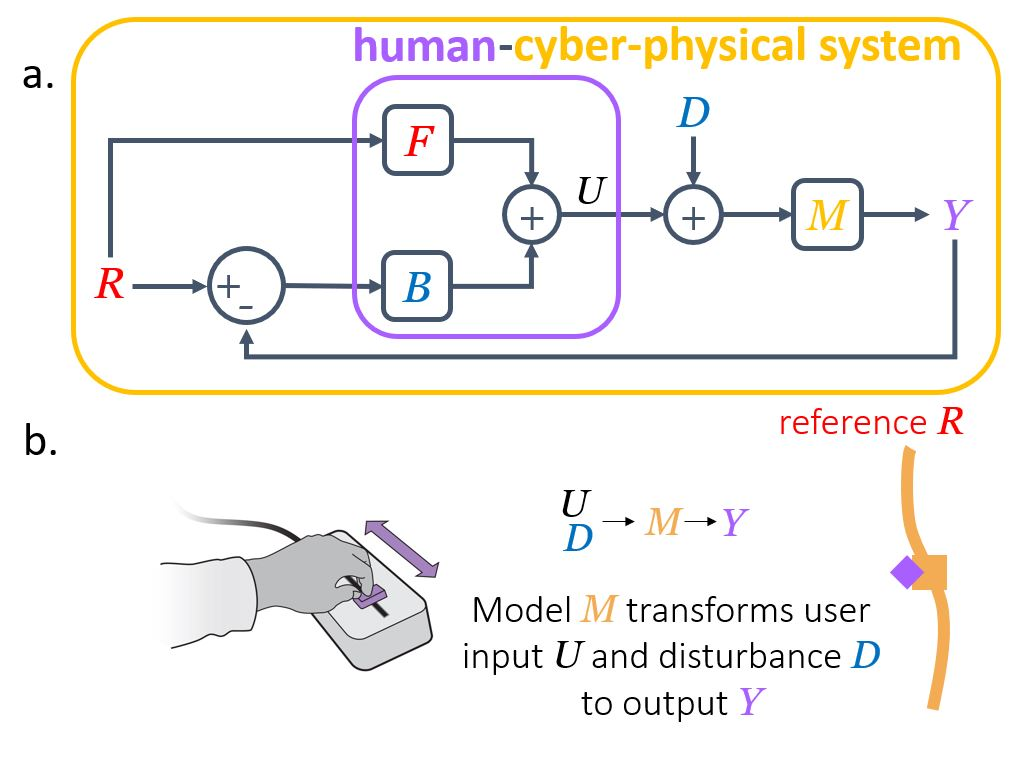
\includegraphics[width=8.4cm]{game.jpg}    % The printed column width is 8.4 cm.
\caption{a. Diagram of human operator playing the game with the slider, and b. block diagram of HCPS} 
\label{fig:game}
\end{center}
\end{figure}

In this experiment, we separated feedforward and feedback control by adding a disturbance $d$ to the user input $u$ such that the user must use only feedback control to mitigate the effect of $d$ on $y$ (Fig.~\ref{fig:game} b).

\subsection{Separation of Feedforward and Feedback Control Inputs}

Feedforward controller $F$ and feedback controller $B$ can be described in the frequency domain by, 

\begin{equation} \label{eq:B}
{B=\frac{-H_{DU}}{M(1+H_{DU})}},
\end{equation}
\begin{equation} \label{eq:F}
{F=H_{RU}(1+BM)},
\end{equation}

where $H_{RU}$ represents the transfer function that maps $r$ in the frequency domain $R$ to $U$, and $H_{DU}$ is the transfer function that maps $D$ to $U$. These controllers can be obtained for each frequency at which we present a reference and a disturbance to the operator. It was obtained by representing $U$ as a linear combination of $F$ and $B$ with prescribed ($R, M, D$) values, 

\begin{equation} \label{eq:U}
{U=\frac{F+B}{1+BM}R-\frac{BM}{1+BM}D},
\end{equation}

and by setting $H_{RU}=\frac{U}{R}$ and $H_{DU}=\frac{U}{D}$, the equations for $F,B$ in Eqns.~\ref{eq:B}, \ref{eq:F} can be obtained.

\section{Experimental Design}
\subsection{Overview of Experimental Setup}

An Arduino Due in conjunction with a 10 $k\Omega$ potentiometer slider was used to apply a model $M$ such that the input from the slider was transformed to the output such that $y=mu$. A scaled and shifted sum of sines was used to create the reference and disturbance trajectories, with the signal at all prime numbers starting from 2 to ensure no harmonic signals. Three types of assays were presented to the operator - 1. only $r$, with $d=0$, 2. only $d$, with $r=0$, and 3. $r+d$, with each at alternating frequencies such that for one frequency, either $r=0$ or $d=0$. The $d$ only trials differed from the $r$ only trials by the $r$ trajectory having a look-ahead and past of 0.25 seconds, whereas the $d$ trajectory had no look-ahead that the operator could use to determine an optimal input $u$. The phase shifts were randomized for each trial, and the three assays were presented in sequence as follows: 
\begin{center}
1. $r+d \times 2$ trials\newline
2. $d \times 10$ trials\newline
3. $r+d \times 2$ trials\newline
4. $r \times 10$ trials\newline
5. $r+d \times 10$ trials\newline
\end{center}

Two models were presented sequentially to observe model inversion in a simpler first-order (fo) model and a more complex second-order (so) model, with,
\begin{equation} \label{eq:Mfo}
{m_{fo}: \dot{y}=u, }
\end{equation} 
\begin{equation} \label{eq:Mso}
{m_{so}: \ddot{y}-\dot{y}=u}
\end{equation} 

\subsection{Experimental Data Analysis}

Seven participants were recruited to track the yellow trajectory with the purple cursor on the screen. Data was analyzed with Python 2.7.3 in the frequency domain by taking the fast fourier transform (FFT) of measured and known values $FFT(u,m,r,d,y)=U,M,R,D,Y$ for each trial. Coherence was calculated between the $r,d$ and $r+d$ trials, as well as $H_{DU}$ and $H_{RU}$ to assess linearity of the HCPS. A Wilcoxon Signed Rank test was performed to determine the extent to which the medians of $H_{DU}$ and $H_{RU}$ from the $d,r$ trials are similar to the values calculated from the $r+d$ trials. 

A feedback only model and a feedback and feedforward model was fitted to the trials to determine whether feedback and feedforward model had a better fit to the data than the feedback only model. 

$F$ and $B$ were calculated as described in Eqns.~\ref{eq:B}, \ref{eq:F} to determine the extent to which $F$ was similar to the model inverse $M^{-1}$. A Wilcoxon Signed Rank tests was performed to quantify this similarity.

\section{Results}

\subsection{Validation of Linearity of HCPS}
\begin{figure*}[t]
\begin{center}
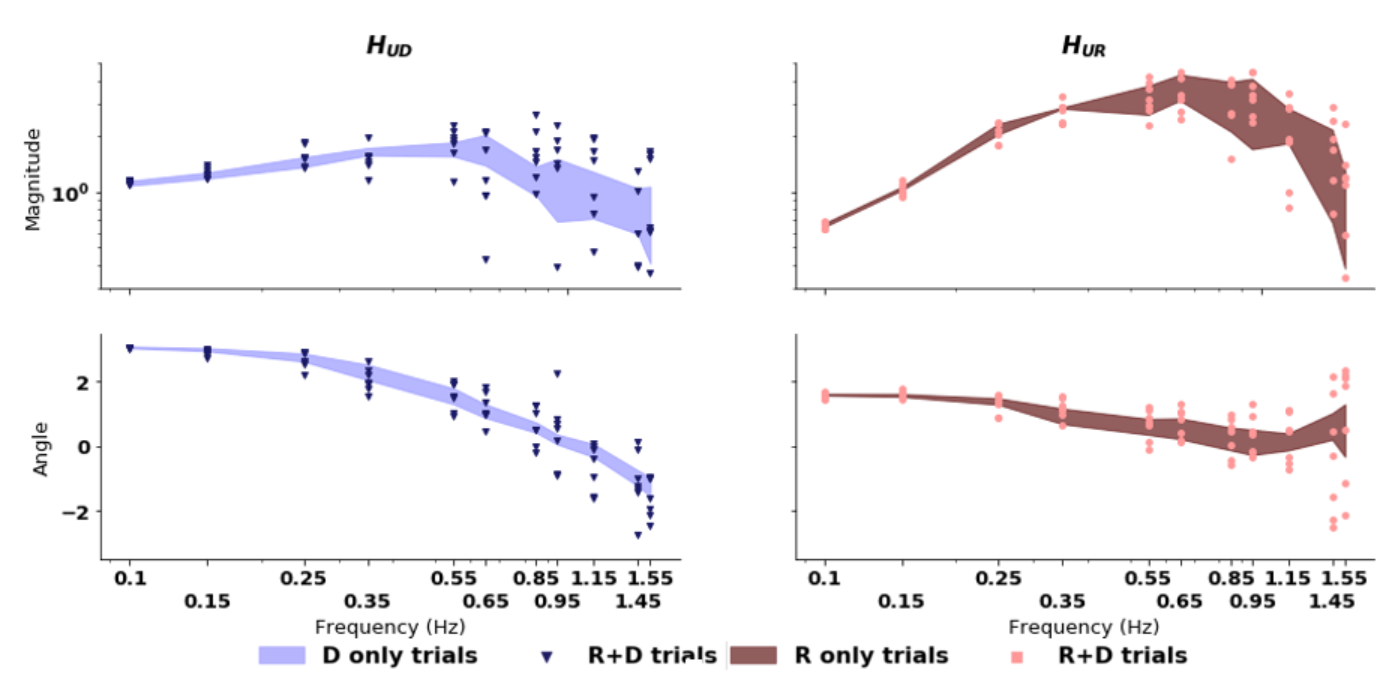
\includegraphics[width=16.8cm]{linearity.jpg}    % The printed column width is 8.4 cm.
\caption{a. Diagram of human operator playing the game with the slider, and b. block diagram of HCPS} 
\label{fig:linearity}
\end{center}
\end{figure*}

The high coherence between the $r$ and $r+d$ trials (median, range $C_{r,r+d} = 0.84, 0.21-1.0$) and $d$ and $r+d$ trials (median, range $C_{d,r+d} = 0.82, 0.10-0.99$) demonstrated that $r+d$ trials may be well predicted from $r$ and $d$ trials by a linear least squares function, suggesting that the HCPS may be linear (Fig.~\ref{fig:linearity}a). Further investigation into the transfer functions $H_{RU}$ and $H_{DU}$ demonstrated a high degree of overlap between the $R$ and $R+D$ trials and $D$ and $R+D$ trials, and the Wilcoxon signed-rank test indicated that with $\alpha<0.05$, there was no statistical difference in $H_{RU}$ and $H_{DU}$ in either average magnitude or angle between the only $R$ or only $D$ trials and the $R+D$ trials. The positive results from this superposition test indicates that the HCPS can be thought of and analyzed as a linear system. 

Something here about FB and FF 

\begin{figure}[h]
\begin{center}

\includegraphics[width=8.4cm]{Capture.png}    % The printed column width is 8.4 cm.
\caption{Fit of feedforward only model and fit of feedforward and feedback model} 
\label{fig:FBvsFF}
\end{center}
\end{figure}

\subsection{Verification of Dynamic Model Inversion for First and Second Order Systems}

The feedback and feedforward estimates pooled across all individuals and trials demonstrate large deviations in magnitude from $M^{-1}$ for the feedforward controller for both $R$ and $R+D$ trials (Fig.~\ref{fig:ffMinv}). The Wilcoxon signed-rank test demonstrated that there was a significant difference between the feedforward controller and $M^{-1}$ (first-order: $p=0.006$, second-order: $p=0.018$). SOMETHING ABOUT THE ANGLES HERE 

Due to the smaller number of trials ran for the $R+D$ trials compared to the $R$ only and $D$ only trials, we saw a much larger IQR for the $R+D$ trials than the $R$ only and $D$ only trials.

\begin{figure}[h]
\begin{center}
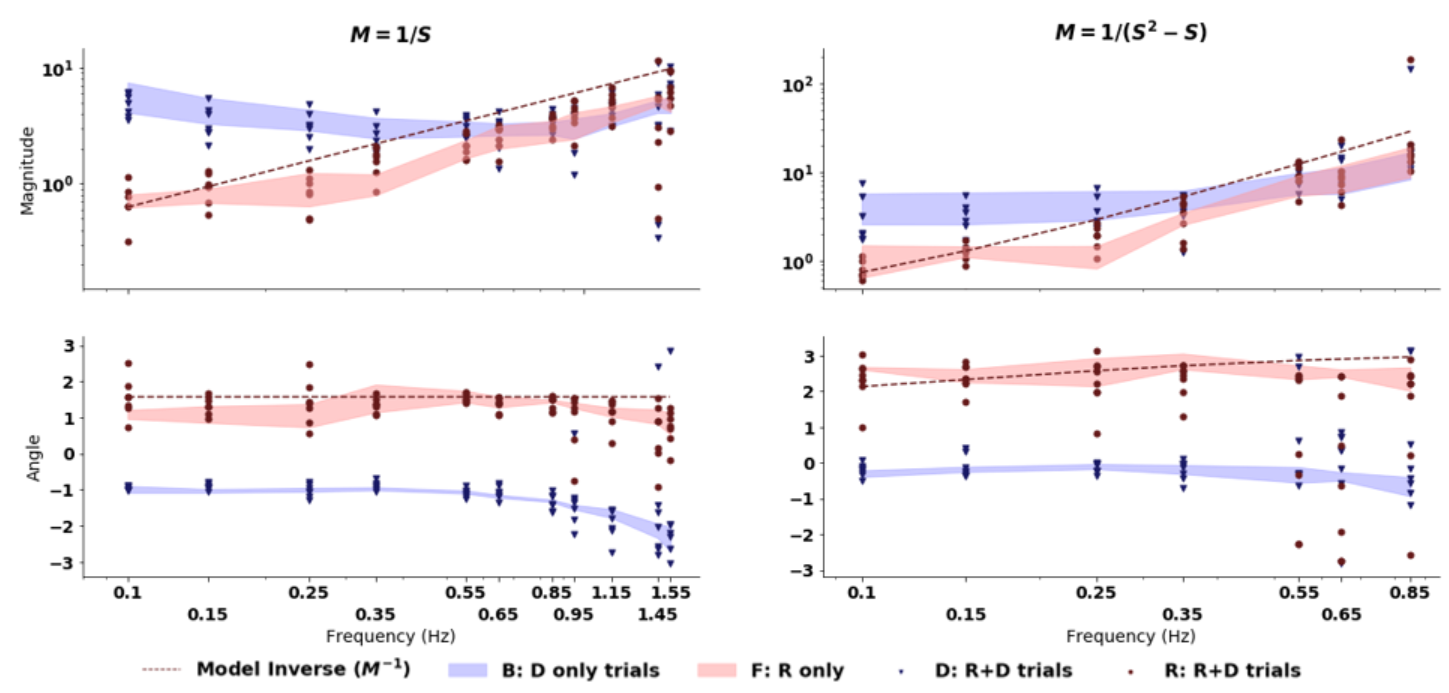
\includegraphics[width=8.4cm]{ffMinv.png}    % The printed column width is 8.4 cm.
\caption{Feedforward block is approximately equal to $M^{-1}$ for both first-order and second-order systems} 
\label{fig:ffMinv}
\end{center}
\end{figure}

\section{Discussion and Conclusion}

A conclusion section is not required. Although a conclusion may review
the main points of the paper, do not replicate the abstract as the
conclusion. A conclusion might elaborate on the importance of the work
or suggest applications and extensions.

\begin{ack}
This research is supported by a grant from the National Science Foundation under the CISE CRII CPS (1565529) and the Washington Research Foundation Funds for Innovation in Neuroengineering.
\end{ack}


\bibliography{ifacconf}             % bib file to produce the bibliography
                                                     % with bibtex (preferred)
\bibliographystyle{ifacconf.bst}
%\begin{thebibliography}{xx}  % you can also add the bibliography by hand

%\bibitem[Able(1956)]{Abl:56}
%B.C. Able.
%\newblock Nucleic acid content of microscope.
%\newblock \emph{Nature}, 135:\penalty0 7--9, 1956.

%\bibitem[Able et~al.(1954)Able, Tagg, and Rush]{AbTaRu:54}
%B.C. Able, R.A. Tagg, and M.~Rush.
%\newblock Enzyme-catalyzed cellular transanimations.
%\newblock In A.F. Round, editor, \emph{Advances in Enzymology}, volume~2, pages
%  125--247. Academic Press, New York, 3rd edition, 1954.

%\bibitem[Keohane(1958)]{Keo:58}
%R.~Keohane.
%\newblock \emph{Power and Interdependence: World Politics in Transitions}.
%\newblock Little, Brown \& Co., Boston, 1958.

%\bibitem[Powers(1985)]{Pow:85}
%T.~Powers.
%\newblock Is there a way out?
%\newblock \emph{Harpers}, pages 35--47, June 1985.

%\bibitem[Soukhanov(1992)]{Heritage:92}
%A.~H. Soukhanov, editor.
%\newblock \emph{{The American Heritage. Dictionary of the American Language}}.
%\newblock Houghton Mifflin Company, 1992.

%\end{thebibliography}
\end{document}
